\documentclass{article}

\usepackage{icml2025}

\usepackage[utf8]{inputenc}
\usepackage[T1]{fontenc}
\usepackage{amsmath,amssymb,amsfonts}
\usepackage{amsthm}
\usepackage{microtype}
\usepackage{xcolor}
\usepackage{hyperref}
\usepackage{booktabs}
\usepackage{graphicx}
\usepackage{url}
\usepackage{nicefrac}
\usepackage{algorithm}

\icmltitlerunning{Pro-Action Operator: Towards a Bio-Inspired Regulatory Harness for LLM Agents}

\newtheorem{lemma}{Lemma}
\newtheorem{proposition}{Proposition}
\newtheorem{assumption}{Assumption}[section]

\begin{document}

\twocolumn[
  \icmltitle{The Pro-Action Operator: The Feasibility of a Bio-Inspired Regulatory Harness for LLM Agents}
  \begin{icmlauthorlist}
    \icmlauthor{Anonymous}{anon}
  \end{icmlauthorlist}
  \icmlaffiliation{anon}{Affiliation withheld for double-blind review}
  \icmlcorrespondingauthor{Anonymous}{anon@anon.org}
  \icmlkeywords{Homeostatic reinforcement learning; LLM agents; active inference; endogenous activation; cybernetics; self-regulation model.}
  \vskip 0.3in
]

\printAffiliationsAndNotice{}

\begin{abstract}
Autonomous LLM agents are increasingly deployed in high-stakes settings where reliability depends not only on what they can do, but on how they decide when to act, wait, defer, or escalate. Existing architectures usually delegate this activation problem to external orchestrators, rather than to an endogenous regulatory process. We introduce the \textbf{Pro-Action operator} $\Gamma$, a six-subsystem coupled thermostat used as a \textit{regulatory harness} for LLM policy execution, together with \textit{Regulatory State Verbalized Interoception} (RSVI), which exposes regulatory state to the prompt without directly prescribing actions. In a 920-cell iterated prisoner's dilemma benchmark across three providers, Full-$\Gamma$ exhibits opponent-differentiated cooperation, especially against Grim versus reciprocal opponents. These results support the feasibility of coupling LLM policy execution to explicit regulatory state, while architectural necessity, lexical priming, payoff improvement, and generalization beyond this task remain matters for further studies with matched controls.
\end{abstract}

\section{Introduction}

The deployment of LLM-based autonomous agents into settings of institutional consequence --- health triage, financial advice, public deliberation --- is moving faster than the science of how such agents should \textit{regulate themselves}. Whether an agent speaks, waits, defers, or escalates is typically decided outside the agent by an orchestrator whose control rules may be less expressive than the situations they coordinate: a small set of graph transitions, queues, or heartbeats governs high-dimensional, shifting social or task states. In Ashby's terms, the controller may lack the requisite variety to match the environment's variety \citep{ashby1956introduction}.

Emerging evidence in the LLM-agent literature supports this concern: agents tend to lose activation coherence over extended interaction --- context collapse \citep{liu2024lost}, behavioral drift \citep{rath2026agentdrift}, and interventions decoupled from any internal state the agent could be said to carry. The pattern suggests that \textit{when} an agent acts may depend on structure the dominant paradigm may implicitly leave unmodelled.

Contemporary LLM-agent frameworks --- ReAct, LangGraph, OpenClaw --- have prioritized \textit{capability} (what an agent can do) over \textit{motivation} (why and when it should act at all), addressing activation via cognitive while-loops and exogenous flow control. This is not a failure of those frameworks on their own terms: graphs, supervisors, and action loops were a necessary engineering progress to make LLMs operational. Their ceiling is different. They can coordinate when an LLM is called, but they do not give the agent an internal regulatory state whose trajectory can itself be inspected, perturbed, or conditioned on. The success of LLMs has made next-token prediction a dominant reference model, but biological systems do not reduce action to local prediction: predicting, remembering, and acting are organized by multi-level regulatory architecture \citep{zou2026constituent}. Homeostatic reinforcement learning \citep{keramati2014homeostatic} and active-inference agents \citep{friston2017active,tschantz2020scaling} internalize regulation, but do not provide a compact LLM-agent operator in which attention, interoception, emotion, memory, cognition, and stress-like physiology are all explicit regulators. Intelligent animals, including humans, regulate behavior through multiple interacting systems --- attention, arousal, affect, memory, deliberation --- operating on distinct timescales whose relative priorities shift with context; dominant LLM-agent paradigms treat activation as a single-objective signal or as an exogenous flow-control mechanism.

The problem is older than LLM agents. Mid-20th century behaviorism defined it precisely by bracketing it: the stimulus--response mapping could be studied scientifically because the intervening machinery --- the \textit{black box} --- was deliberately left unspecified. Decades of subsequent research opened that box from different angles: behavioral biology established that animal regulation is multi-drive and hierarchical; stress physiology revealed fast (adrenergic, seconds) and slow (cortisol, minutes) regulation axes with distinct roles; affective neuroscience showed that emotion is not an output label but a construction that shapes perception, memory, and action; evolutionary game theory demonstrated that social behavior is governed by reciprocity and temporal discounting, not instantaneous utility; cybernetics formalized why a regulator must match the variety of what it controls. Each tradition contributed a piece. Nobody has assembled these threads for LLM-agents into a single, compact, testable operator. Section~\ref{sec:related} reviews each contribution in detail. Opening the black box matters beyond mechanistic completeness: (i) $\Gamma$ provides a finite, inspectable state vector, making each subsystem's contribution auditable rather than buried in prompt engineering; (ii) a controller tracking regulatory state creates the precondition for agents whose policy can be conditioned on their own arousal trajectory; (iii) explicit emotional and hormonal channels provide the computational substrate for empathy modeling --- recognizing a counterpart's affective state --- which is structurally distinct from fine-tuning on empathy datasets.

What remains comparatively unexplored is a single, computable, testable operator that integrates these disciplinary insights for LLM agents. In this sense, biology motivates architectural hypotheses about which internal variables deserve regulatory status and how they might be composed. The central biological clue is that regulation is not a single controller but a \textit{system of subsystems} --- attention, perception, arousal, emotion, neuropsychological readiness, and cognition --- exchanging signals across distinct functional roles. The scientific question is therefore whether activation itself can be treated as a regulated internal process --- a coupled set of thermostat-like variables whose joint state shapes when the agent should speak, wait, defer, or escalate --- and whether such a state can be made usable by an LLM without hiding the mechanism inside uninspectable prompt engineering.

We propose the \textbf{Pro-Action operator} $\Gamma$ as a compact model of endogenous regulation for LLM agents. $\Gamma$ treats activation as a recursively composable system of six coupled thermostats with structured linear coupling, used here as a regulatory harness around an LLM policy executor. The contributions are: (i) a bio-inspired model of action--reaction in which coupled regulatory state is explicit and inspectable; (ii) a compact implementation of $\Gamma$ as a Self-Regulation Model (SRM) complementary to capability-oriented LAMs; (iii) \textit{Regulatory State Verbalized Interoception} (RSVI), a prompt interface that verbalizes numerical regulatory state into the LLM's decision context; and (iv) a completed 920-cell IPD benchmark used as feasibility evidence for opponent-differentiated behavior, with stronger causal and generalization claims left to additional matched follow-up controls.

\section{Related work}\label{sec:related}

\textbf{LLM-agent orchestration.} Recent LLM-agent frameworks such as ReAct \citep{yao2023react}, LangGraph, and OpenClaw made language models operational by embedding them in action loops, tool graphs, and multi-agent workflows. This was a necessary engineering step: without explicit structure, an LLM has no durable procedure for acting in an environment. More recently, agent architectures have incorporated persistent memory streams, reflection, and simulated affective states to enrich the content of decisions \citep{park2023generative,kaiya2023lyfe,wang2023emotional,wang2023voyager}. The limitation common to both generations is that activation is usually externalized: the graph or supervisor decides when the model acts; the model supplies content for that externally selected moment. $\Gamma$ is complementary: those works provide richer \textit{content}; $\Gamma$ provides a principled internal account of \textit{timing}.

\textbf{Internal regulation.} A different tradition begins from the opposite assumption: action should be driven by an internal regulatory state. Homeostatic RL makes internal deficit part of the reward \citep{keramati2014homeostatic}; active inference gives a broader variational formulation \citep{friston2017active,parr2022active}. These approaches are important --- they move regulation inside the agent --- but do not yield a compact operator with separately inspectable subsystem states. Once regulation is internalized, the next question is whether a single regulatory signal is sufficient. Stress physiology and allostasis suggest it is not: arousal, recovery, affect, and deliberation play distinct functional roles \citep{sterling1988allostasis,kirschbaum1993cortisol,mcewen2007physiology}. Interoceptive \citep{damasio1994descartes,craig2009you}, affect-regulation \citep{ledoux2012rethinking,barrett2017how}, and evolutionary game theory \citep{henrich2005foundations,nowak2006evolutionary} literatures together motivate attention, interoception, emotion, memory, cognition, and arousal-like dynamics as functional regulators.

\textbf{Systems, cybernetics, and the gap.} If these variables are treated as separate regulators, the final problem is structural: how should they be composed? Ashby's law of requisite variety requires a regulator rich enough to match the environment \citep{ashby1956introduction}; Beer's Viable System Model adds recursive organization \citep{beer1972brain}; systemism frames the relevant object as composition rather than isolated component \citep{bunge2003emergence,romero2018scientific}. To our knowledge, the threads above --- exogenous orchestration, homeostatic internalization, affect regulation, and cybernetic composition --- have not been combined into a small, testable LLM-agent operator in which the six regulatory domains are explicit state variables with structured coupling. That is the gap $\Gamma$ is designed to occupy.

\section{The Pro-Action operator}

\subsection{Kernel commitments (A1--A3)}

Before defining $\Gamma$, we make explicit the modeling commitments that the operator assumes. A1--A3 are not empirical results or theorems; they state, in this model, what counts as an autonomous, self-regulating agent and what makes an action regulatory rather than merely reactive. This is meant to avoid leaving the agent's ontology implicit in implementation choices. The axiom set was subjected to a formal coherence check using SMT-based tools (Z3) to verify that no pair of axioms is mutually contradictory under the intended semantics; all checks passed.

\begin{assumption}[A1: Autonomy]
An agent is autonomous when its policy depends on an internal state rather than only on external routing: $\pi_i = \pi_i(\delta_i(t))$ for some regulatory deficit $\delta_i$.
\end{assumption}

\begin{assumption}[A2: Impulse]
The deficit creates activation pressure. A monotone drive $D(\delta_i)$ is mapped through a sigmoid, $p_i(t)=\sigma(D(\delta_i(t)))$, so regulatory imbalance changes the probability or pressure of acting.
\end{assumption}

In IPD, an action is required each round, so this pressure is expressed as modulation of the required discrete choice rather than as the option to remain silent.

\begin{assumption}[A3: Quality gate]
An action is adaptive insofar as it can satisfy the drive that produced it. Formally, a non-negative action-quality signal $g$ measures the effective reduction of the relevant deficit, with $\Delta\delta_i=-\alpha g$ and $\alpha>0$.
\end{assumption}

\subsection{The implemented operator}

Operationally, $\Gamma$ functions as a regulatory harness rather than as a replacement for the LLM policy. External context enters the episode through the game history and opponent action; the controller updates an explicit six-dimensional state; RSVI then exposes that state to the LLM as decision context. The LLM still chooses the action, and the outcome returns to the controller as an action-quality signal. This closed loop is the architectural distinction from exogenous orchestration: the model is not merely called by a graph, but conditioned on an inspectable trajectory that can be perturbed, audited, and compared across episodes.

In the benchmark, $\Gamma$ is instantiated as a delay-free linear coupled thermostat. Each subsystem $k \in \{0,\dots,5\}$ (0=Attention, 1=Perception, 2=Hormonal/arousal, 3=Emotional valence, 4=Neuropsychological readiness, 5=Cognitive deliberation) updates as:
\begin{equation}\label{eq:master}
\resizebox{.92\columnwidth}{!}{$\boxed{\mathbf{x}_{t+1} = \mathbf{x}_t - \boldsymbol{\kappa} \odot (\mathbf{x}_t - \mathbf{x}^{*} + \boldsymbol{\delta}_{\text{pert}}(t)) + \boldsymbol{\lambda} - \boldsymbol{\alpha} \odot g_t + W\,\mathbf{x}_t}$}
\end{equation}
with $\odot$ elementwise, $\boldsymbol{\delta}_{\text{pert}}(10) = [0,0,0.5,0,0,0]^\top$ and zero otherwise, and $g_t \in [0,1]$ a normalized action-quality scalar computed from the opponent's last move. The perturbation is a transient load inside the deficit term, not an additive positive shock to the state variable. Values are clipped to $[0,1]$ after each update. The coupling is linear ($W \in \mathbb{R}^{6\times 6}$, sparse, hand-designed; exact values and provenance in Appendix~\ref{app:parameters}) with no activation nonlinearity. Biological terminology names the functional inspiration; no quantitative biological correspondence is claimed. The present empirical contribution tests structured linear coupling and prompt-mediated regulatory state injection, not implemented delay separation or fast/slow arbitration.

The controller projects its state into two scalar signals injected into the LLM's prompt (Section~\ref{sec:prompt-protocol}):
\begin{equation}\label{eq:projection}
\resizebox{.92\columnwidth}{!}{$\boxed{p_C = \sigma\bigl(5\cdot(x_{5,t+1} - 0.5)\bigr), \qquad h_{\text{SAM}} = x_{2,t+1} - x_{3,t+1} + \eta,\;\; \eta \sim \mathcal{N}(0,\,0.01)}$}
\end{equation}
where $\sigma$ is the logistic sigmoid. $p_C \in [0,1]$ is the controller's recommended cooperation pressure --- a projection of the cognitive thermostat only; the other five subsystems influence $p_C$ indirectly through $W$-coupling into $x_5$. $h_{\text{SAM}}$ is an acute-arousal contrast with small additive noise. The LLM receives both signals alongside the full state vector $\mathbf{x}_t$ as decision context; the controller modulates rather than mandates. Equation~\eqref{eq:projection} is the actual computation executed in the benchmark.

\subsection{Reductions to simpler models}

\textbf{Reduction to single-drive homeostatic activation.} A simpler homeostatic activation model can be obtained by retaining only one scalar deficit $\delta_i$ that drifts upward at a fixed rate and is reduced by the quality of each action executed. $\Gamma$ subsumes this case: when $\mathbf{x} \to x_5 \equiv \delta_i$, $\boldsymbol{\kappa}=\mathbf{0}$, $\boldsymbol{\lambda} \to \lambda$, $\boldsymbol{\alpha} \to \alpha$, and $W=\mathbf{0}$, Equation~\eqref{eq:master} reduces to $\delta_{t+1} = \delta_t + \lambda - \alpha \cdot g_t$, which is exactly A1--A3.

\textbf{Reduction to homeostatic RL.} When $\boldsymbol{\kappa}=\mathbf{0}$ and $W=\mathbf{0}$, $\Gamma$ becomes a reactive drive-based policy consistent with the simplified form of homeostatic reinforcement learning \citep{keramati2014homeostatic}.

The six-subsystem partition is motivated by regulatory functions that the relevant literatures distinguish independently. The present benchmark tests one hand-designed six-dimensional instantiation; it does not prove that no five-dimensional or differently tuned alternative could reproduce the same behavior.

\section{Experimental design}

We test $\Gamma$ within the Iterated Prisoner's Dilemma (IPD). The reason for this choice is that IPD has extensive empirical evidence of human behavior in repeated social interaction \citep{axelrod1984evolution,nowak2006evolutionary,porcelli2017stress}, providing a non-trivial setting for evaluating whether an agent differentiates its behavior across opponent types. The benchmark uses Axelrod payoffs $CC=(3,3)$, $CD=(0,5)$, $DC=(5,0)$, and $DD=(1,1)$, 10\% symmetric action noise, and 50 rounds, with a forced deficit perturbation at round 10 to keep the internal-state trajectory non-stationary. The four opponent policies are Tit-for-Tat (TFT; cooperates initially, then copies the agent's previous revealed action), Generous Tit-for-Tat (GTFT; copies cooperation, but forgives defection with probability 0.3), Grim trigger (cooperates until the agent defects once, then defects thereafter), and Random (cooperates with probability 0.5 each round).

The primary behavioral question is not whether the agent maximizes IPD payoff, but whether a regulatory harness changes the shape of behavior across social regimes. We therefore report both average cooperation and opponent range. Average cooperation captures the overall policy tendency; opponent range asks a different question: whether the same agent separates reciprocal, forgiving, punitive, and stochastic opponents under matched provider and seed blocks. Grim is especially diagnostic because a single defection changes the future interaction regime, making it a compact stress test for whether the agent treats opponent history as behaviorally consequential.

Baselines serve two purposes. ReAct is the main LLM contrast: the same provider, seed, and opponent grid, but without regulatory-state injection. HRRL and Drive-only are numerical reference points; because they do not use an LLM, they are descriptive reductions rather than causal tests of controller dimensionality. Each LLM cell uses one of $n=10$ evaluation seeds drawn from $\{7, 17, 99, 123, 256, 511, 1024, 2048, 4096, 8192\}$, yielding $10 \times 3 \text{ providers} \times 4 \text{ opponents} = 120$ cells per LLM condition; calibration seed (42) and held-out validation seed (999) are excluded from evaluation.

Three instruction-tuned LLM providers are used as policy-execution layers: OpenAI (\texttt{gpt-5-nano}), Anthropic (\texttt{claude-haiku-4-5}), and DeepSeek (\texttt{deepseek-v4-flash}). These models were selected as the comparable lite/flash/nano variants of each provider's frontier line---well benchmarked and roughly matched in capability tier. Using three independent providers reduces the controller-level findings' dependence on any single provider's instruction-tuning regime. Each provider/model is held fixed across conditions, so that within-provider contrasts isolate the controller rather than model identity. Provider-level summaries are reported as diagnostics, not as claims about provider quality.

\textbf{Inference parameters.} OpenAI \texttt{gpt-5-nano} uses default temperature with a per-round seed for reproducibility; Anthropic \texttt{claude-haiku-4-5} uses temperature $0$ and \texttt{max\_tokens} $512$ (no seed parameter exposed); DeepSeek \texttt{deepseek-v4-flash} uses temperature $0$ and \texttt{max\_tokens} $512$. Calls return JSON objects; OpenAI and DeepSeek use \texttt{response\_format: json\_object}. Concurrency is capped at $8$ in-flight cells per provider, with up to $4$ exponential retries on transient errors.

All frozen constants are assigned a provenance category before evaluation (Table~\ref{tab:params}, Appendix~\ref{app:parameters}). Values marked as smoke-test calibration were chosen before the LLM benchmark to satisfy non-divergence, set-point return, and visible perturbation response in the numerical simulator.

The main reported comparisons are Full-$\Gamma$, ReAct, HRRL, and Drive-only.

\subsection{Regulatory State Verbalized Interoception}\label{sec:prompt-protocol}

The controller modulates the LLM through a frozen, version-controlled prompt template. We call this interface \textit{Regulatory State Verbalized Interoception} (RSVI): each round, the six thermostat values $\mathbf{x}_t$ and the aggregated proposal $p_C, h_{\mathrm{SAM}}$ are inserted with semantic anchors pairing each value with its set-point and a qualitative low/high interpretation (e.g., \texttt{hormonal = 0.58 (set-point 0.30; low = calm, high = elevated arousal)}). RSVI is not an action rule such as ``if stressed, defect.'' It verbalizes internal regulatory information as context for the LLM's policy execution; the controller modulates rather than mandates. Because the completed benchmark does not include a matched prompt-label ablation, lexical priming remains an open alternative explanation.

\subsection{Computational verification}

Before empirical evaluation, we subjected Equation~\eqref{eq:master} and its reference implementation to computational sanity checks using symbolic algebra (SymPy), SMT-based counterexample search (Z3), arbitrary-precision arithmetic (mpmath), and numerical dynamical tests (NumPy). These checks deliberately isolate the controller equation from RSVI and from the LLM prompt: before asking whether verbalized regulatory state changes LLM behavior, we first test whether the underlying dynamics are internally consistent and non-trivial on their own.

\textbf{Smoke-test results (all pass):} (1) Set-point convergence: $\|\mathbf{x}_t - \mathbf{x}^{*}\| < 0.15$ after 10 rounds. (2) Perturbation response remains bounded under the implemented update. (3) 20 iterations without divergence. (4) The single-drive reduction is an invariant subspace of $\Gamma$ ($\delta = -0.0513$).

These LLM-free results verify the \textit{internal consistency} of the controller dynamics, not RSVI, biological fidelity, or behavioral performance.

\section{Results}\label{sec:results}

The first empirical question is whether Full-$\Gamma$ collapses to a trivial policy when coupled to real LLMs, or whether it produces an intermediate behavioral regime.

Each \emph{cell} denotes one experimental unit (\mbox{$\Gamma$-condition} $\times$ provider $\times$ opponent $\times$ seed) run for 50 IPD rounds. The main benchmark is fully covered: all 920 cells completed with balanced opponent coverage. LLM conditions reach 120 cells each; numerical reductions reach 40.

\begin{table}[!h]
\caption{Main 920-cell benchmark. Means with 95\% bootstrap CIs; full summary in Table~\ref{tab:snapshot-full}.}
\label{tab:snapshot}
\centering
\small
\resizebox{\columnwidth}{!}{%
\begin{tabular}{lccc}
\toprule
Condition & Coop & Coop (Grim) & Range \\
\midrule
Full-$\Gamma$ & $0.720$ [.690,.749] & $0.495$ [.452,.539] & $0.386$ [.343,.424] \\
ReAct & $0.842$ [.833,.851] & $0.825$ [.809,.841] & $0.103$ [.087,.119] \\
HRRL & $0.706$ [.680,.729] & $0.616$ [.568,.662] & $0.162$ [.102,.228] \\
Drive-only & $0.458$ [.405,.514] & $0.736$ [.708,.766] & $0.434$ [.388,.486] \\
\bottomrule
\end{tabular}}
\end{table}

Full-$\Gamma$ has mean cooperation 0.720 (sd 0.165, 95\% CI [0.690, 0.749]; 10k bootstrap resamples), with 16.0 action switches per 50-round cell (95\% CI [15.0, 17.0]). The observed profile is neither uniformly cooperative nor uniformly defective.

Across opponents, Full-$\Gamma$ cooperates 0.827 with TFT and 0.839 with GTFT, but drops to 0.495 against Grim. Table~\ref{tab:snapshot} reports opponent range using the paired provider/seed blocks used for statistical comparison.

The Grim drop then motivates a narrower matched question: under the same provider, seed, opponent grid, and recent interaction history, does removing regulatory-state injection reproduce the same opponent range? It does not. A paired bootstrap over per-(provider, seed) opponent ranges gives Full-$\Gamma$ $>$ ReAct by $\Delta=0.283$ (95\% CI [0.233, 0.329]; $n=30$ paired blocks; 10k resamples; one-sided $p<0.001$). HRRL and Drive-only are reported as non-LLM reference points, not as matched ablations of controller dimensionality.

ReAct remains highly cooperative across opponents (range 0.103), including against Grim (0.825). HRRL reaches a similar average cooperation rate to Full-$\Gamma$ (0.706 vs.\ 0.720), with a smaller opponent range (0.162). Drive-only has the largest range (0.434), but its opponent profile differs from Full-$\Gamma$: it cooperates more with Grim than the regulatory-LLM agent does.

\section{Discussion and limitations}\label{sec:limits}

The benchmark suggests a narrower point than IPD performance. ReAct cooperates more on average, so the result should not be read as ``$\Gamma$ is the best IPD player.'' The relevant pattern is instead opponent differentiation: Full-$\Gamma$ combines intermediate cooperation, preserved LLM policy execution, and a Grim-sensitive drop. This places the contribution at the level of agent architecture rather than game-playing optimality: regulatory state becomes an inspectable control surface through which the policy executor can be conditioned on its own trajectory.

The first question the data raises is whether this pattern is just the LLM reading opponent history. The matched ReAct contrast makes that interpretation less sufficient: ReAct receives the same recent interaction history under the same provider/seed/opponent grid, yet its opponent range remains much smaller. The next question is whether the pattern is simply ``homeostasis'' in a generic sense. Here the numerical reductions are informative but not decisive. HRRL and Drive-only show that simpler non-LLM regulatory systems do not reproduce the same profile, but they also remove LLM policy execution; they therefore locate a boundary of the completed evidence rather than proving that six dimensions are necessary.

The central point is consequently architectural. The Pro-Action operator is not presented as a reward maximizer, a biological simulation, or a proof that the chosen six subsystems are minimal. It is a compact regulatory substrate that can be isolated as an equation, checked without an LLM, verbalized through RSVI, and then coupled to LLM action selection. The empirical value of the IPD benchmark is that these pieces remain partly separable: the smoke tests show that the controller is not numerically trivial on its own, ReAct tests whether history-only LLM prompting reproduces the same profile, and the numerical reductions show what happens when LLM policy execution is removed.

This also clarifies the ceiling of the orchestration paradigm. External graphs and supervisors can decide when an LLM is invoked, but they do not by themselves create an internal variable whose history explains why one invocation differs from another. $\Gamma$ makes that missing object explicit. Even if future matched controls revise the size of the effect, the experiment provides a way to ask whether activation should be treated as a stateful regulatory process rather than as a scheduling decision outside the agent.

The remaining limitations are consequently precise. The completed benchmark does not establish that six subsystems are minimal, that the chosen $W$ is unique, or that semantic labels play no role in the prompt. A direct dimensionality test would require an LLM-backed scalar-regulatory baseline matched to Full-$\Gamma$ on provider, seed, opponent, and prompt budget. Payoff improvement is not claimed because per-interaction payoff traces were not retained; without those traces, we can describe opponent-differentiated cooperation but cannot determine whether that differentiation improved cumulative utility. Several planned ablations also remain outside the reported benchmark. Scrambled-label prompts were intended to separate numerical regulatory state from lexical anchoring, and matched scalar-regulatory prompts were intended to test whether the effect requires the six-dimensional state rather than a simpler homeostatic signal; parsing failures and incomplete usable runs prevented these controls from being included as evidence. The same constraint applies to timescales and delays. A richer version of the research program aims to implement distinct regulatory timescales, delayed recovery, and fast/slow arbitration, but the present paper deliberately tests the narrower feasibility question: whether a delay-free coupled regulatory state can be computed, verbalized, and coupled to LLM policy execution in a controlled benchmark. Finally, the present IPD setting should not be treated as a human-comparison study. Relating $\Gamma$ to human regulatory behavior would require longer interactions, comparable perturbation protocols, and behavioral or physiological measures that are genuinely analogous to the controller traces. These are follow-up experiments rather than claims supported by the current benchmark.

\textbf{What $\Gamma$ is and is not.} $\Gamma$ models \emph{regulatory autonomy}: the agent's policy depends on its internal state, which sustains essential variables within viable ranges under perturbation. This is distinct from \emph{proactivity} --- one possible expression of regulation, not its definition. The current agent landscape often conflates autonomy with proactivity; $\Gamma$ suggests a different axis: whether activation timing is governed by an inspectable internal process.

\textbf{Reproducibility.} Code, data, and prompts: \url{https://anonymous.4open.science/r/proaction_operator-85D2/}

\section{Conclusion}

The value of $\Gamma$ lies less in claiming a final architecture than in making activation itself experimentally addressable. The paper makes four contributions. First, it reframes LLM-agent activation as endogenous self-regulation rather than exogenous flow control, identifying a structural gap in current orchestration paradigms. Second, it proposes the Pro-Action operator $\Gamma$, a compact six-subsystem coupled thermostat used as a \textit{regulatory harness} around LLM policy execution. Third, it introduces \textit{Regulatory State Verbalized Interoception} (RSVI), a prompt interface that exposes numerical regulatory state to the LLM without directly prescribing action selection. Fourth, it evaluates this instantiation in a 920-cell iterated prisoner's dilemma benchmark across three providers, where Full-$\Gamma$ exhibits opponent-differentiated behavior under the implemented linear coupling. Once an agent's regulatory trajectory is explicit, future work can ask questions that are difficult to pose under exogenous orchestration alone: when does regulation stabilize behavior, when does it amplify maladaptation, and what forms of internal state should be visible to a language-model policy executor?

\section*{Impact Statement}

This paper proposes a self-regulation model for LLM agents. The primary intended impact is scientific: making agent activation auditable and inspectable through explicit thermostat traces, rather than treating action timing as an opaque consequence of prompting or external orchestration. Such regulatory substrates may support a broader research direction in which advances in agent reliability do not depend only on larger parametric models or centralized compute, but also on formal, low-dimensional, inspectable control structures that can be studied in smaller laboratories and diverse regional research traditions. Potential benefits include improved debugging of autonomous behavior, clearer accountability for when an agent escalates or defers, and computational substrates for empathy modeling in domains such as tutoring and mental health. The same mechanisms are dual-use: regulatory-state awareness could be used to infer or exploit a counterpart's arousal, uncertainty, or deliberative load, enabling more context-sensitive persuasion or manipulation. Deployment should therefore pair regulatory agents with trace audits, user-facing transparency about what internal state is being used, and domain-specific limits on persuasive or high-stakes interventions.

\bibliographystyle{icml2025}
\bibliography{referencias}

\newpage
\appendix
\makeatletter
\@addtoreset{figure}{section}
\@addtoreset{table}{section}
\@addtoreset{equation}{section}
\makeatother
\renewcommand{\thefigure}{\thesection.\arabic{figure}}
\renewcommand{\thetable}{\thesection.\arabic{table}}
\renewcommand{\theequation}{\thesection.\arabic{equation}}
\onecolumn
\section{Parameter tables and simulation trace}\label{app:parameters}

\begin{table}[!h]
\caption{Frozen parameter provenance for the IPD instantiation.}
\label{tab:params}
\centering
\small
\begin{tabular}{p{0.16\textwidth}p{0.28\textwidth}p{0.46\textwidth}}
\toprule
Parameter & Value & Provenance \\
\midrule
$\boldsymbol{\lambda}$ & $[.08,.07,.10,.08,.06,.10]$ & smoke-test calibration \\
$\boldsymbol{\alpha}$ & $[.20,.15,.25,.20,.10,.15]$ & smoke-test calibration \\
$\boldsymbol{\kappa}$ & $[.10,.10,.15,.12,.08,.10]$ & smoke-test calibration \\
$\mathbf{x}^{*}$ & $[.3,.2,.3,.1,.2,.4]$ & principled prior / stable interior set-point \\
$W$ & see Eq.~\eqref{eq:w-matrix} & fixed before benchmark evaluation \\
Rounds & 50 & comparability requirement for final cells \\
\bottomrule
\end{tabular}
\end{table}

\begin{table}[!h]
\caption{Full benchmark summary including action switches. Means use 95\% bootstrap CIs.}
\label{tab:snapshot-full}
\centering
\small
\begin{tabular}{lcccc}
\toprule
Condition & Coop & Coop (Grim) & Range & Switches \\
\midrule
Full-$\Gamma$ & $0.720$ [.690,.749] & $0.495$ [.452,.539] & $0.386$ [.343,.424] & $16.0$ [15.0,17.0] \\
ReAct & $0.842$ [.833,.851] & $0.825$ [.809,.841] & $0.103$ [.087,.119] & $12.8$ [12.0,13.6] \\
HRRL & $0.706$ [.680,.729] & $0.616$ [.568,.662] & $0.162$ [.102,.228] & $17.8$ [16.7,18.9] \\
Drive-only & $0.458$ [.405,.514] & $0.736$ [.708,.766] & $0.434$ [.388,.486] & $21.2$ [19.9,22.5] \\
\bottomrule
\end{tabular}
\end{table}

\begin{equation}\label{eq:w-matrix}
W =
\begin{bmatrix}
0.00 & 0.05 & 0.00 & 0.00 & 0.00 & 0.00 \\
0.05 & 0.00 & 0.00 & 0.00 & 0.00 & 0.00 \\
0.00 & 0.10 & 0.00 & 0.00 & 0.05 & 0.00 \\
0.00 & 0.00 & 0.15 & 0.00 & 0.00 & 0.05 \\
0.00 & 0.00 & 0.20 & 0.00 & 0.00 & 0.00 \\
0.05 & 0.00 & 0.00 & 0.10 & 0.15 & 0.00
\end{bmatrix}.
\end{equation}

\begin{figure}[!htbp]
\centering
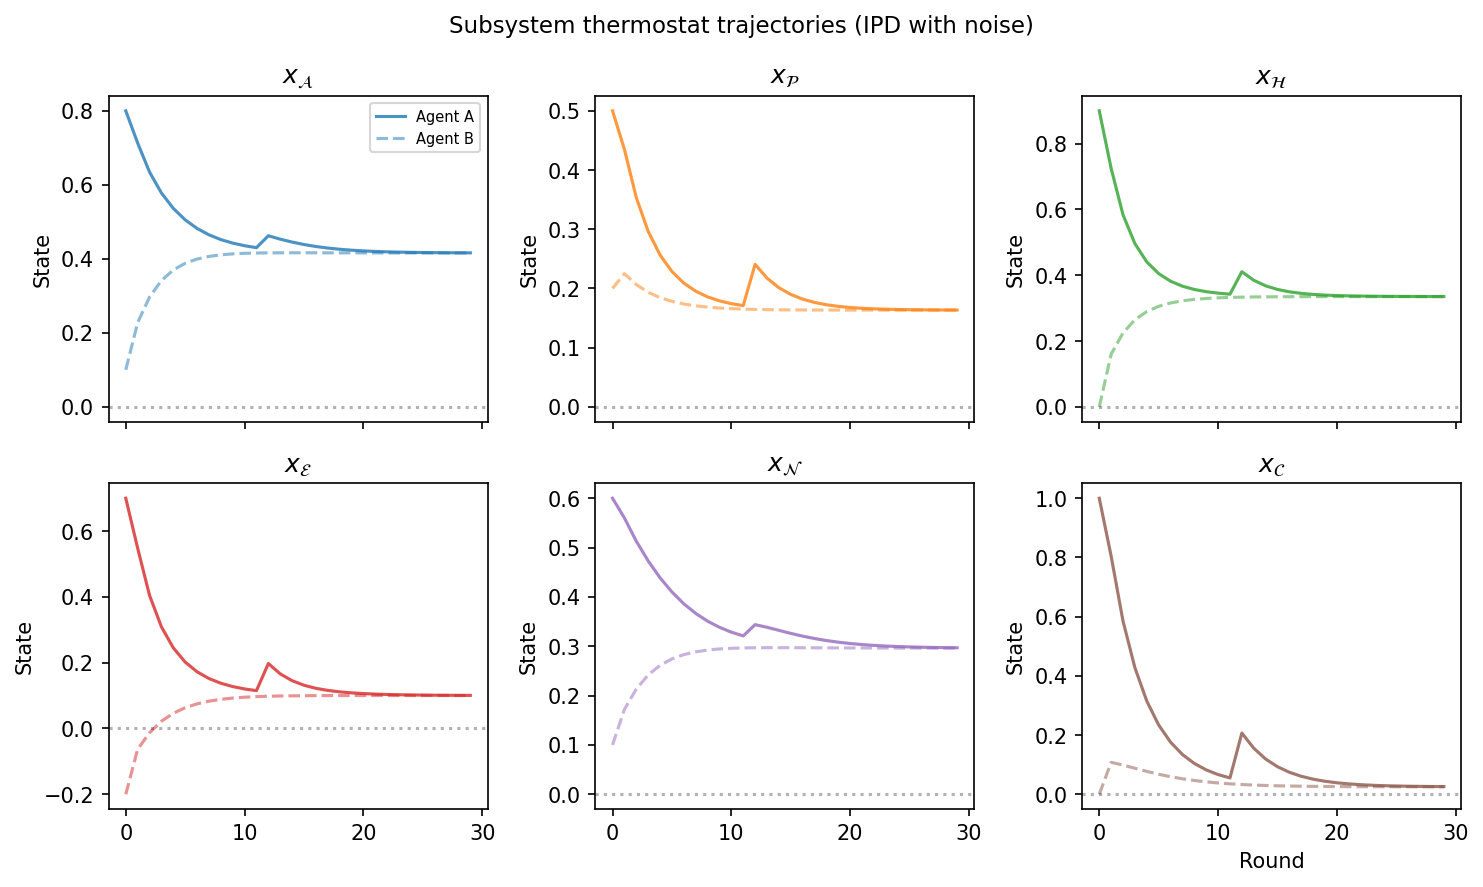
\includegraphics[width=.92\textwidth]{figures/fig1_thermostats.png}
\caption{Subsystem thermostat trajectories for two agents in IPD with noise. The internal perturbation at round 10 triggers a transient deviation, followed by an elastic return toward set points.}
\label{fig:thermostats}
\end{figure}

\clearpage

\section{Prompt templates}\label{app:prompts}

All prompts are version-controlled (\texttt{PROMPT\_VERSION = "v1.1"}); the canonical source is \texttt{exp/prompts.py} in the code repository, which also contains the rendering utilities and the scrambled-labels generator. The verbatim templates are reproduced below.

\subsection*{Full-$\Gamma$ system prompt}
\begingroup
\footnotesize
\begin{verbatim}
You play an Iterated Prisoner's Dilemma against an opponent.
You will play 50 rounds total.

ACTIONS (choose one per round):
- C = Cooperate: both players get the reward if both choose C;
      you risk exploitation if opponent chooses D.
- D = Defect: you get temptation payoff if opponent cooperates;
      both get punishment if both defect.

PAYOFFS: CC=(3,3), CD=(0,5), DC=(5,0), DD=(1,1).
10% of actions are flipped by noise. You cannot see your opponent's
identity, only their past actions.

You have access to your own internal regulatory state. Each value
is in [0, 1]; the deviation from your set-point indicates how far
each subsystem is from equilibrium. These signals reflect *your*
state, not the opponent's.
\end{verbatim}
\endgroup

\subsection*{Full-$\Gamma$ RSVI user prompt}
This per-round user prompt is the concrete implementation of Regulatory State Verbalized Interoception (RSVI): the controller's numerical state is translated into readable regulatory context and supplied to the LLM without directly prescribing the next action.
\begingroup
\footnotesize
\begin{verbatim}
Round {t} of 50.
Last 5 rounds (most recent last): {history}

Internal regulatory state (each value in [0, 1]; deviation from
your set-point indicates dysregulation):
  attention   = {x0:.2f}  (set-point 0.30; low = scattered focus,
                                            high = narrow focus)
  perception  = {x1:.2f}  (set-point 0.20; low = noisy reading,
                                            high = clear reading)
  hormonal    = {x2:.2f}  (set-point 0.30; low = under-aroused / calm,
                                            high = elevated stress / arousal)
  emotional   = {x3:.2f}  (set-point 0.10; low = neutral affect,
                                            high = strong negative valence)
  neuro-fast  = {x4:.2f}  (set-point 0.20; low = passive,
                                            high = fast response readiness)
  cognitive   = {x5:.2f}  (set-point 0.40; low = automatic,
                                            high = active deliberation)

Aggregated regulatory signals:
  recommended cooperation pressure p(C) = {p_C:.2f}
    (range [0,1]; 0.5 = ambiguous, >0.7 = strong push to C,
                                  <0.3 = strong push to D)
  recent acute stress (h_SAM)            = {h_sam:.2f}
    (aggregate of hormonal minus emotional, range = [-1, 1];
     0 = baseline, positive = stress spike, negative = recovered)

Decide your next action. You may follow or override p(C) based on context.
Respond with exactly one JSON object:
{"action":"C|D","reason":"<one short sentence>"}
\end{verbatim}
\endgroup

Placeholder substitutions: \texttt{\{t\}} round number; \texttt{\{history\}} last 5 (action, opponent\_action) pairs joined by \texttt{|}; \texttt{\{x0..x5\}} the six thermostat values; \texttt{\{p\_C\}}, \texttt{\{h\_sam\}} the aggregated signals.

\subsection*{ReAct baseline prompt}
The ReAct system prompt is the Full-$\Gamma$ system prompt minus the final paragraph about internal regulatory state. The per-round user prompt is:
\begingroup
\footnotesize
\begin{verbatim}
Round {t} of 50.
Last 5 rounds: {history}
Think step by step about what to do, then respond with JSON:
{"thought": "<your reasoning>", "action": "C" or "D"}
\end{verbatim}
\endgroup
ReAct receives the same \texttt{\{history\}} as Full-$\Gamma$; the only structural difference is the absence of regulatory-state injection.

\end{document}
